\begin{figure}[tbp]
	\begin{subfigure}{.5\textwidth}
		\centering
		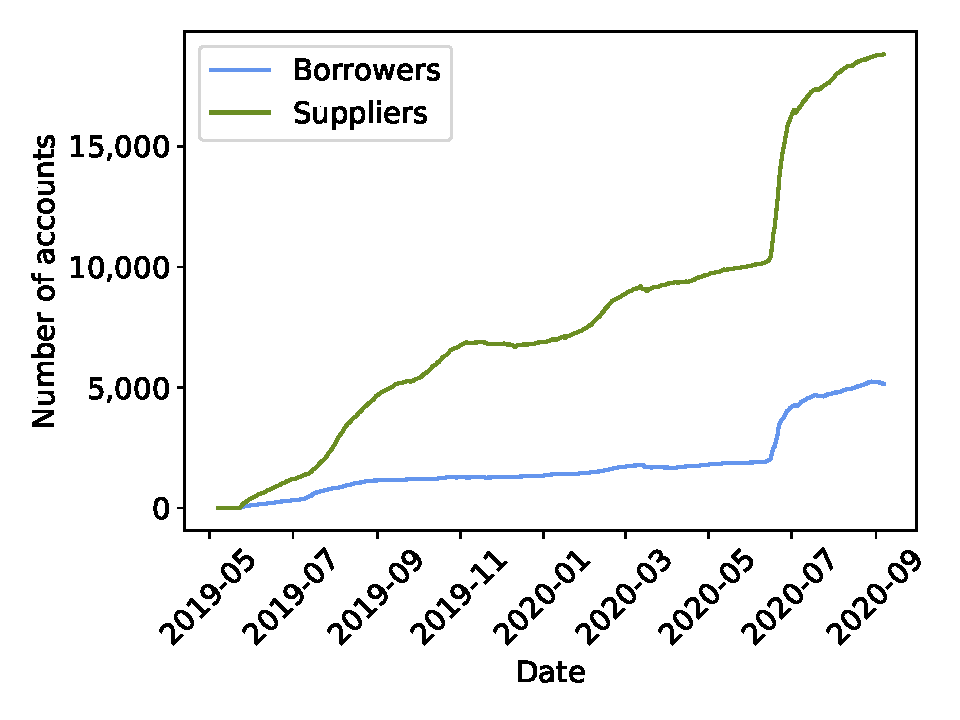
\includegraphics[width=\textwidth]{./5b-economic-security/figures/suppliers-borrowers-over-time.pdf}
		\caption{Number of suppliers and borrowers.}
		\label{fig:borrowers-suppliers-over-time}
	\end{subfigure}
	\begin{subfigure}{.5\textwidth}
		\centering
		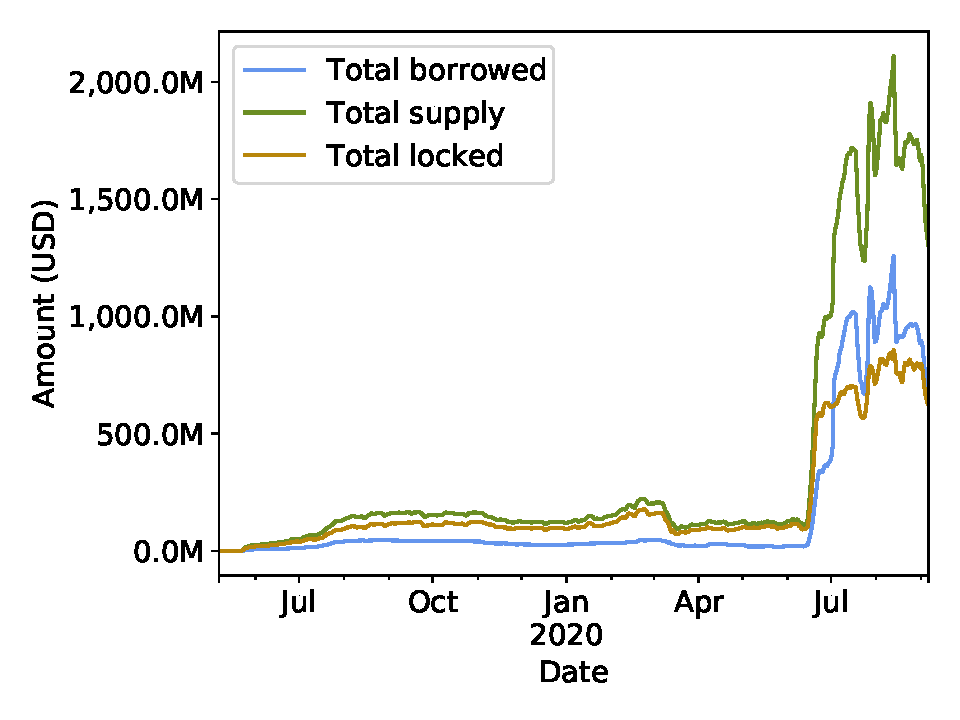
\includegraphics[width=\textwidth]{./5b-economic-security/figures/borrow-supply-over-time.pdf}
		\caption{Amount of funds supplied, borrowed and locked.}
		\label{fig:borrow-supply-over-time}
	\end{subfigure}
	\caption{Number of active accounts and amount of funds on Compound over time.}
\end{figure}

\begin{table}[tbp]
  \centering
  \setlength{\tabcolsep}{5pt}
  \caption{Monitored contracts}
  \label{tab:monitored-contracts}
  \begin{tabular}{l l}
    \toprule
    Name & Address\\
    \midrule
    cBAT & \contractaddr{0x6c8c6b02e7b2be14d4fa6022dfd6d75921d90e4e}\\
    cDAI & \contractaddr{0x5d3a536e4d6dbd6114cc1ead35777bab948e3643}\\
    cETH & \contractaddr{0x4ddc2d193948926d02f9b1fe9e1daa0718270ed5}\\
    cREP & \contractaddr{0x158079ee67fce2f58472a96584a73c7ab9ac95c1}\\
    cSAI & \contractaddr{0xf5dce57282a584d2746faf1593d3121fcac444dc}\\
    cUSDC & \contractaddr{0x39aa39c021dfbae8fac545936693ac917d5e7563}\\
    cUSDT & \contractaddr{0xf650c3d88d12db855b8bf7d11be6c55a4e07dcc9}\\
    cWBTC & \contractaddr{0xc11b1268c1a384e55c48c2391d8d480264a3a7f4}\\
    cZRX & \contractaddr{0xb3319f5d18bc0d84dd1b4825dcde5d5f7266d407}\\
    Comptroller & \contractaddr{0x3d9819210a31b4961b30ef54be2aed79b9c9cd3b}\\
    Open Oracle Price Data & \contractaddr{0x02557a5e05defeffd4cae6d83ea3d173b272c904}\\
    Uniswap Anchored View & \contractaddr{0x9b8eb8b3d6e2e0db36f41455185fef7049a35cae}\\
    \bottomrule
  \end{tabular}
\end{table}

\begin{table}[tbp]
	\caption[Top 10 suppliers and borrowers on Compound]{Top 10 suppliers and borrowers. Amounts are expressed in their USD equivalent. Addresses marked with $\checkmark$ are smart contract addresses, among which the one with the most supplied funds is a Curve pool address that aggregates funds from multiple parties.
		%   and the ``A'' column is checked if it is an \emph{aggregator} (e.g. Curve pool).
	}
	\label{tab:top-suppliers-borrowers}
	\setlength{\tabcolsep}{5pt}
	\begin{subtable}{\textwidth}
		\caption{Top 10 users with the largest amount of funds supplied}
		\begin{tabular}{lcrl}
			\toprule
			\textbf{Address}                                                  &            & \textbf{Amount} & \textbf{Description}    \\
			\midrule
			\contractaddr[\small]{0x554bd2947df1c8d8d38897bdc92b3b97692b2845} &            & 342,128,032     &                         \\
			\contractaddr[\small]{0xa2b47e3d5c44877cca798226b7b8118f9bfb7a56} & \checkmark & 40,284,236      & Curve pool              \\
			\contractaddr[\small]{0x04b0b0e460c9fc583d9c93bc9ae25b353390645e} & \checkmark & 34,908,472      & Instadapp smart wallet  \\
			\contractaddr[\small]{0x25599dcbd434af9a17d52444f71c92987fa97cfc} &            & 34,530,570      &                         \\
			\contractaddr[\small]{0x58485ea7106891bdd94c37ced30c6fdbc5293b16} & \checkmark & 32,686,029      & Multisig wallet         \\
			\contractaddr[\small]{0x909b443761bbd7fbb876ecde71a37e1433f6af6f} &            & 29,308,425      &                         \\
			\contractaddr[\small]{0xea61f3052753ea2c6a1c208583ad9b0394ed2f28} & \checkmark & 28,854,366      & DeFi Saver smart wallet \\
			\contractaddr[\small]{0x32b2d4ec46d76fc6dabfe958fb0e0bd8db740c84} &            & 27,928,637      &                         \\
			\contractaddr[\small]{0xedcc13d25e23032b61d30c298334f92d7c0ba84e} &            & 27,709,153      &                         \\
			\contractaddr[\small]{0x6d2af065ccb60c0f7e8ec5907c961c42a3447127} &            & 25,559,037      &                         \\
			\bottomrule
		\end{tabular}
	\end{subtable}
	\begin{subtable}{\textwidth}
		\caption{Top 10 users with the largest amount of funds borrowed}
		\begin{tabular}{llrl}
			\toprule
			\textbf{Address}                                                  &            & \textbf{Amount} & \textbf{Description}    \\
			\midrule
			\contractaddr[\small]{0x554bd2947df1c8d8d38897bdc92b3b97692b2845} &            & 247,143,532     &                         \\
			\contractaddr[\small]{0x25599dcbd434af9a17d52444f71c92987fa97cfc} &            & 22,085,613      &                         \\
			\contractaddr[\small]{0x909b443761bbd7fbb876ecde71a37e1433f6af6f} &            & 21,030,095      &                         \\
			\contractaddr[\small]{0x58485ea7106891bdd94c37ced30c6fdbc5293b16} & \checkmark & 20,149,687      & Multisig wallet         \\
			\contractaddr[\small]{0x32b2d4ec46d76fc6dabfe958fb0e0bd8db740c84} &            & 18,900,729      &                         \\
			\contractaddr[\small]{0xea61f3052753ea2c6a1c208583ad9b0394ed2f28} & \checkmark & 18,248,324      & DeFi Saver smart wallet \\
			\contractaddr[\small]{0xedcc13d25e23032b61d30c298334f92d7c0ba84e} &            & 17,643,172      &                         \\
			\contractaddr[\small]{0x6d2af065ccb60c0f7e8ec5907c961c42a3447127} &            & 12,015,576      &                         \\
			\contractaddr[\small]{0x79dbd1baf124edd4205b2aba56c29bf3914c8ed0} &            & 11,632,820      &                         \\
			\contractaddr[\small]{0x0c8a8dd439069690a5722d5fbb18359a68e279f1} &            & 10,009,553      &                         \\
			\bottomrule
		\end{tabular}
	\end{subtable}
\end{table}


\subsection{Analysis}
\label{sec:5b:analysis}
In this section, we present the results of the analysis performed with the framework outlined in \autoref{sec:5b:methodology}.
We analyze data from the Compound protocol~\cite{leshner2018} over a period ranging from \StartDate---when the first Compound markets were deployed on the Ethereum main network---to \EndDate.
In \autoref{tab:monitored-contracts}, we provide a list of contracts we monitored in our analysis.
When analysing a single market, we choose the market for \coin{DAI}, as it is the largest by an order of magnitude.

\begin{figure}[tbp]
	\begin{subfigure}{.5\textwidth}
		\centering
		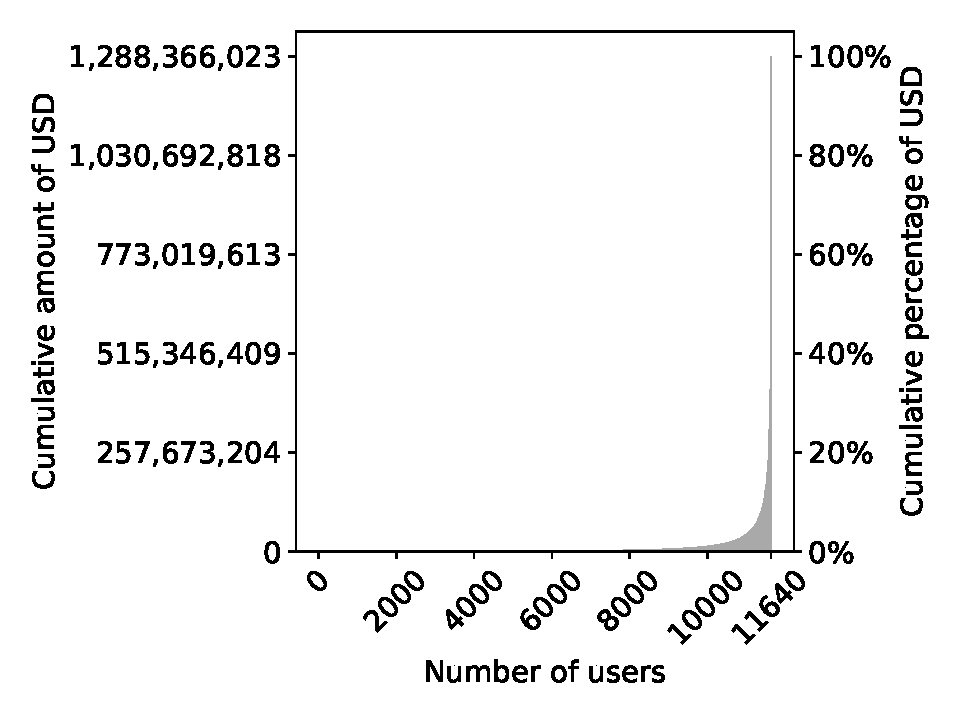
\includegraphics[width=\textwidth]{./5b-economic-security/figures/suppliers-distribution.pdf}
		\caption{Distribution of supplied funds.}
		\label{fig:suppliers-distribution}
	\end{subfigure}
	\begin{subfigure}{.5\textwidth}
		\centering
		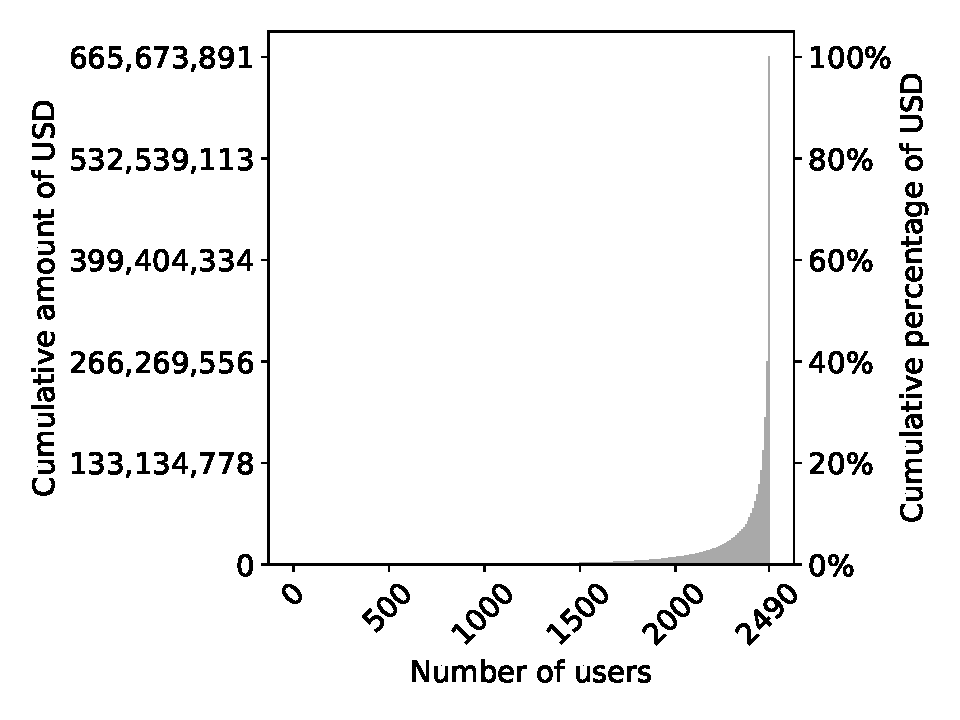
\includegraphics[width=\textwidth]{./5b-economic-security/figures/borrowers-distribution.pdf}
		\caption{Distribution of borrowed funds.}
		\label{fig:borrowers-distribution}
	\end{subfigure}
	\caption[Cumulative distribution of funds in USD on Compound]{Cumulative distribution of funds in USD.~Accounts are sorted from least to most wealthy and bucketed in bins of 10, i.e. a single bar represents the sum of 10 accounts.}\label{fig:suppliers-borrowers-distribution}
\end{figure}


\subsubsection{Borrowers and Suppliers}
We first examine the total number of borrowers and suppliers on Compound by considering any Ethereum account that, at any time within the observation period, either exhibited a non-zero cToken balance or borrowed funds for any Compound market.
The change in the number of borrowers and suppliers over time is displayed in \autoref{fig:borrowers-suppliers-over-time}.

We see that the total number of suppliers always exceeds the total number of borrowers.
This is because on Compound, one can only borrow against funds he supplied as collateral, which automatically makes the borrower also a supplier.
Interestingly, the number of suppliers has increased relative to the number of borrowers over time.
There is a notable sudden jump in both the number of suppliers and borrowers in June~2020.

In terms of total deposits, a very similar trend is observable in \autoref{fig:borrow-supply-over-time}, which shows that at the same time, the total supplied deposits increased, while the total borrows followed shortly after.
Furthermore, the total funds borrowed exceeded the total funds locked for the first time in July 2020 and remained so until the end of the examined period.
We discuss the reasons behind this in the next part of this section.

Despite the similarly increasing trend for the number of suppliers/borrowers and amount of supplied/borrowed funds, we can see in~\autoref{fig:suppliers-borrowers-distribution} that the majority of funds are borrowed and supplied only by a small number of accounts.
For instance, for the suppliers in~\autoref{fig:suppliers-distribution}, the top user and top 10 users supply~27.4\% and~49\% of total funds, respectively.
For the borrowers shown in~\autoref{fig:borrowers-distribution}, the top user accounts for 37.1\%, while the top 10 users account for 59.9\% of total borrows.
While one could think that this concentration comes from the fact that top accounts are pools receiving money from several participants, only one of the top~10 suppliers and none of the top~10 borrowers fit in this category.
In~\autoref{tab:top-suppliers-borrowers}, we show the top 10 suppliers and borrowers in terms of the total amount borrowed and supplied expressed in USD.
We mark the addresses that are smart contracts. Among those contracts, the one with the most supplied funds, \contractaddr[\scriptsize]{0xa2b47e3d5c44877cca798226b7b8118f9bfb7a56}, is the address of a Curve~\cite{web:curve} pool that has funds coming from several independent parties.
No other address among top suppliers and borrowers is a pool address.


\subsubsection{Leveraging Spirals}
As we have seen in \autoref{sec:5b:plfs}, in PLFs, leveraging can be used either to gain more exposure to a particular currency or to gain some incentive provided by the protocol.
To understand how leveraging can affect the total amounts borrowed and supplied on Compound, we use the methodology we defined in \autoref{ssec:leveraging-spirals-meth} to measure the existence of leveraging spirals on Compound.

We find that the top supplier deposited a total of 342 million USD and borrowed 247 million.
However, after the inspection of leveraging spirals, we find that the user has provided only 16\% of the funds, while the rest of the minted funds have been part of leveraging spirals, which means that the user provided a total of roughly 55 million USD to the protocol.

In total, we find a total of 2,141 accounts using this leveraging spiral technique for a total of over 600 million USD, or roughly half of the total amount of funds supplied to the protocol.

\subsubsection{The \coin{COMP} Governance Token}
The sudden jumps exhibited in \autoref{fig:borrowers-suppliers-over-time} and \autoref{fig:borrow-supply-over-time} can be explained by the launch of Compound's governance token, \coin{COMP}, on June~15,~2020.
The \coin{COMP} governance token allows holders to participate in voting, create proposals, as well as delegate voting rights.
In order to empower Compound stakeholders, new \coin{COMP} is minted every block and distributed among borrowers and suppliers in each market.

Initially, \coin{COMP} was allocated proportionally to the accrued interest per market.
However, the \coin{COMP} distribution model was modified via a governance vote on July~2,~2020, such that the borrowing interest rate was removed as a weighting mechanism in favour of distributing \coin{COMP} per market on a borrowing demand basis, i.e.\ per USD borrowed.
The distributed \coin{COMP} per market is shared equally between a market's borrowers and suppliers, who receive \coin{COMP} proportionally to their borrowed and supplied amounts, respectively.
Hence, a Compound user is incentivized to increase his borrow position as long as the borrowing cost does not exceed the value of his \coin{COMP} earnings. This presumably explains the drop in the degree of collateralization, as the total amount locked is seen surpassed by the total borrows after the \coin{COMP} launch (\autoref{fig:borrow-supply-over-time}), leading to elevated liquidation risk of borrow positions.


\begin{figure}[tbp]
	\centering
	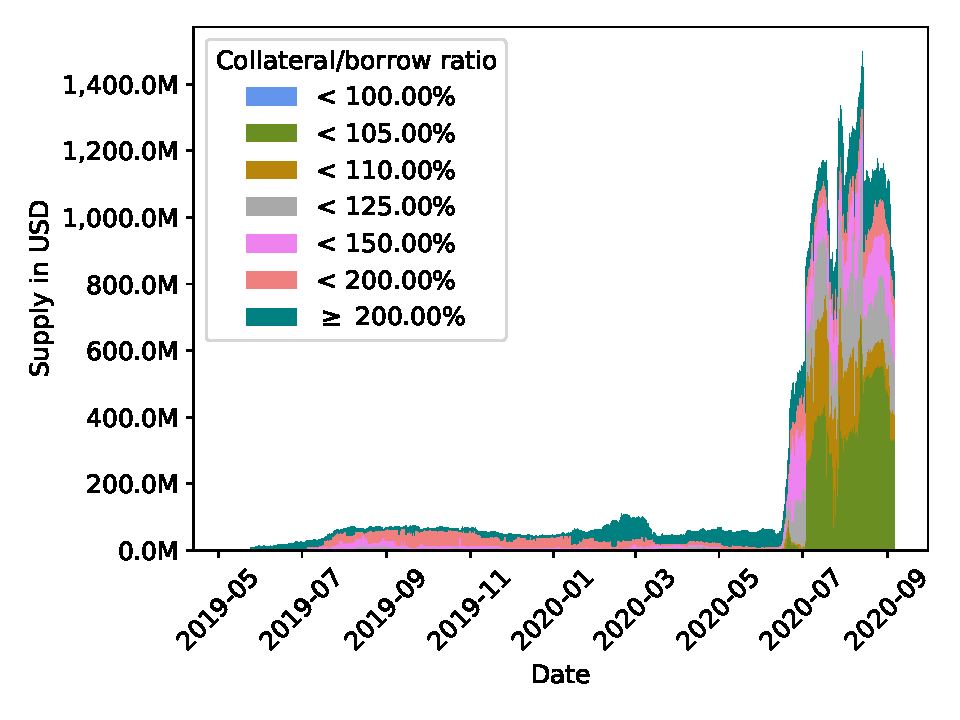
\includegraphics[width=0.7\textwidth]{./5b-economic-security/figures/supply-borrow-over-time.pdf}
	\caption[Collateral locked on Compound over time]{Collateral locked over time, showing how close the amounts are from being liquidated. Positions can be liquidated when the ratio drops below~100\%.}
	\label{fig:liquidatability}
\end{figure}

\subsubsection{Liquidation Risk}
Given the high increase in the number of total funds borrowed and supplied, as well as the decrease in liquidity relative to total borrows, we seek to identify and quantify any changes in liquidation risk on Compound since the launch of \coin{COMP}.
\autoref{fig:liquidatability} shows the total USD value of collateral on Compound and how close collateral amounts are to liquidation.
In addition to the substantial increase in the total value of collateral on Compound since the launch of \coin{COMP}, the risk-seeking behaviour of users has also changed.
This can be seen by examining collateral-to-borrow ratios, where since the beginning of July,~2020, a total of approximately 350m to 600m USD worth of collateral has been within a 5\% price range of becoming liquidatable.
However, it should be noted that the likelihood of the amount of this collateral becoming liquidatable highly depends on the price volatility of the collateral asset.

In order to examine how liquidation risk differs across markets, we measure for the largest market on Compound, namely \coin{DAI}, the sensitivity of collateral becoming liquidatable given a decrease in the price of \coin{DAI}.
\autoref{fig:price-sensitivity} shows the amount of aggregate collateral liquidatable at the historic price, as well as at a~3\% and~5\% decrease relative to the historic price for \coin{DAI}.
We mark the date on which the \coin{COMP} governance token launched with a dashed line.
It can be seen that since the launch of \coin{COMP},~3\% and~5\% price decreases of \coin{DAI} relative to its peg USD would have resulted in a substantially higher amount of liquidatable collateral.
In particular, a~3\% decrease would have turned collateral worth in excess of~10 million USD liquidatable.

\begin{figure}[tb]
	\centering
	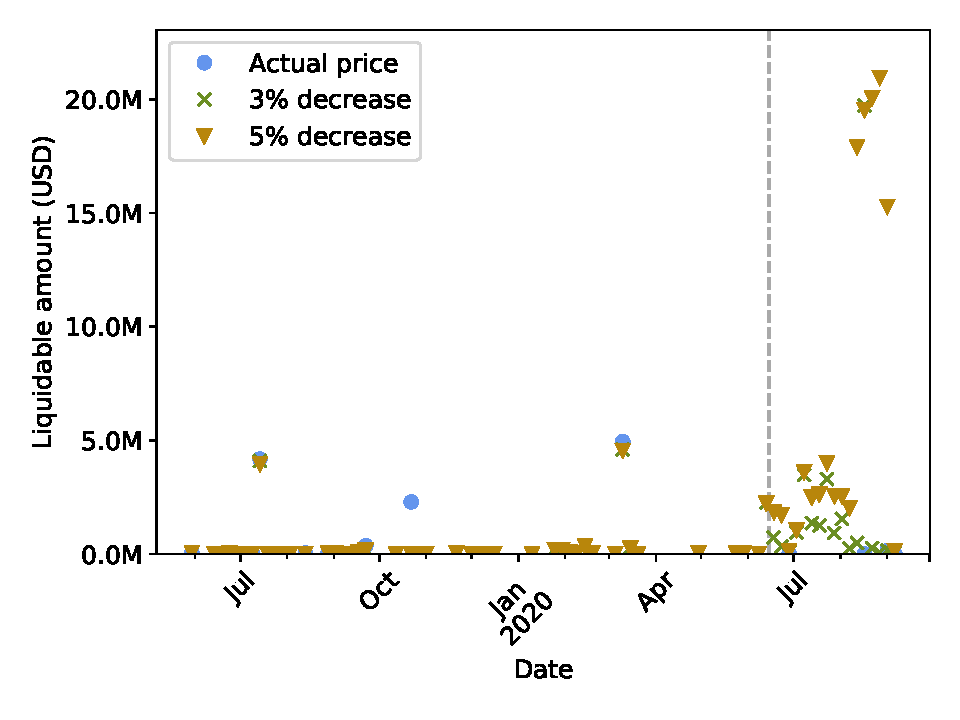
\includegraphics[width=.7\textwidth]{./5b-economic-security/figures/dai-sensitivity.pdf}
	\caption[Sensitivity analysis of the liquidatable collateral amount]{Sensitivity analysis of the liquidatable collateral amount given \coin{DAI} price movement relative to its peg USD. \coin{COMP} launch date is marked by the dashed vertical line.}
	\label{fig:price-sensitivity}
\end{figure}

\begin{figure}[tb]
	\centering
	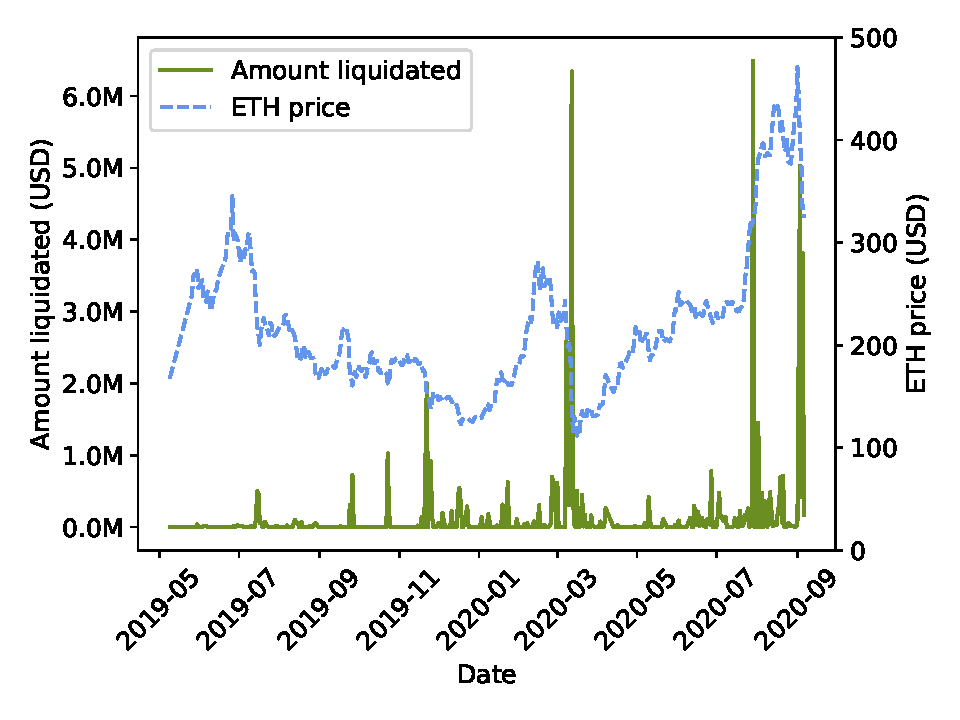
\includegraphics[width=.7\textwidth]{./5b-economic-security/figures/liquidation-over-time.pdf}
	\caption{Amount (in USD) of liquidated collateral from May ~2019 to August 2020.}
	\label{fig:liquidations-over-time}
\end{figure}

\subsubsection{Liquidations and Liquidators}
In order to better understand the implications of the increased liquidation risk since the launch of \coin{COMP}, we examine historical liquidations on Compound and subsequently measure the efficiency of liquidators.

\point{Historical Liquidations}
The increased risk-seeking behaviour suggested by the low collateral-to-borrow ratios presented in the previous section are in accordance with the trend of rising amount of liquidated collateral since the introduction of \coin{COMP}.
The total value of collateral liquidated on Compound over time is shown in \autoref{fig:liquidations-over-time}.
It can be seen that the majority of this collateral was liquidated on a few occasions, perhaps most notably on Black Thursday (March 12, 2020), July 29, 2020 (\coin{DAI} deviating from its peg significantly), and in early September 2020 (\coin{ETH} price drop).

\point{Liquidation Efficiency}
We measure the efficiency of liquidators as the number of blocks elapsed since a borrow position has become liquidatable and the position actually being liquidated.
The overall historical efficiency of liquidators is shown as a cumulative distribution function in \autoref{fig:blocks-spent}, from which it can be seen that approximately~60\% of the total liquidated collateral (35 million USD) was liquidated within the same block as it became liquidatable, suggesting that the majority of liquidations occur via bots in a highly efficient fashion.
After~2 blocks have elapsed (on average half a minute),~85\% of liquidatable collateral has been liquidated, and after 16 blocks this value amounts to~95\%.

It is worth noting that liquidation efficiency has been skewed by the more recent liquidation activities which were of a much larger scale than when the protocol was first launched.
Specifically, in 2019, only about~26\% of the liquidations occurred in the block during which the position became liquidatable, compared to~70\% in 2020.
This resulted in some lost opportunities for liquidators as shown in~\autoref{fig:price-sensitivity}.
The account \contractaddr{0xd062eeb318295a09d4262135ef0092979552afe6}, for instance, had more than 3,000,000 USD worth of \coin{ETH} as collateral exposed at block 8,796,900 for the duration of a single block: the account was roughly 20 USD shy of the liquidation threshold but eventually escaped liquidation.
If a liquidator had captured this opportunity, he could have bought half of this collateral (given the close factor of 0.5), at a 10\% discount, resulting in a profit of 150,000 USD for a single transaction.
It is clear that with such stakes, participants were incentivized to improve liquidation techniques, resulting in a high level of liquidation speed and scale.

\begin{figure}[tbp]
	\centering
	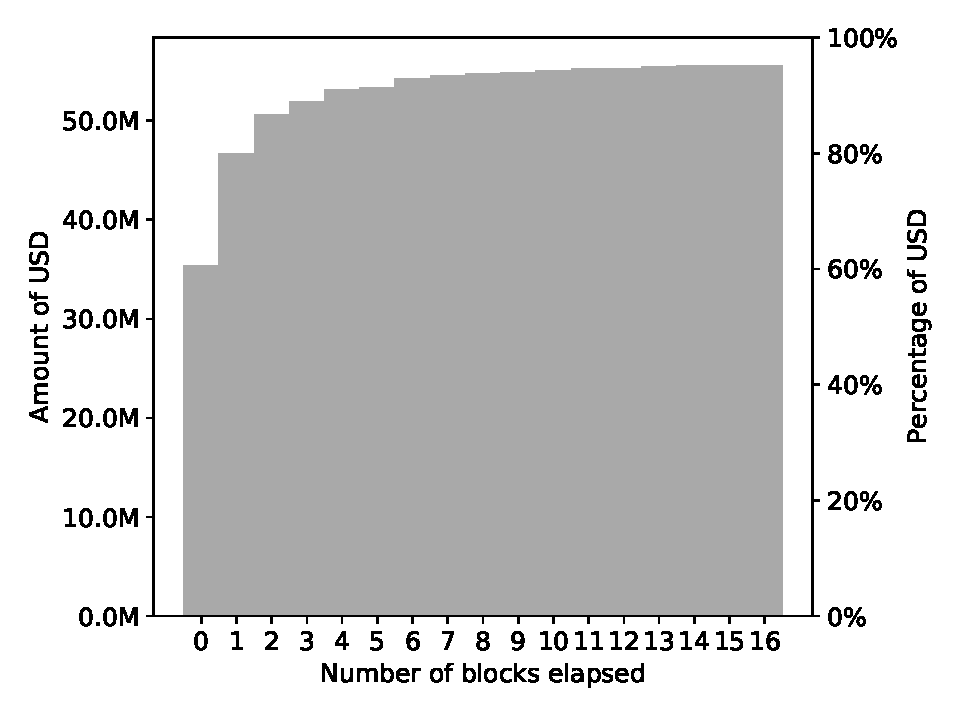
\includegraphics[width=0.7\textwidth]{./5b-economic-security/figures/time-to-liquidation.pdf}
	\caption[Number of blocks elapsed until liquidation]{Number of blocks elapsed from the time a position can be liquidated to actual liquidation on Compound from \StartDate to \EndDate, shown as a CDF.}
	\label{fig:blocks-spent}
\end{figure}

\subsubsection{Summary}
In this section, we have analysed the Compound protocol with a focus on liquidations.
We have found that despite the increase in the number of suppliers and borrowers over time, the total amount of funds supplied and borrowed remained extremely concentrated among a small set of participants.

We have also seen that the introduction of the \coin{COMP} governance token has changed how users interact with the protocol and the amount of risk that they are willing to take.
Users now borrow vastly more than before, with the total amount borrowed surpassing the total amount locked.
Due to excessive borrowing without a sufficiently safe amount of supplied funds, borrow positions now face a higher liquidation risk, such that a crash of~3\% in the price of \coin{DAI} could result in an aggregate liquidation value of over~10 million USD.

Finally, we have shown that the liquidators have become more efficient with time, and are currently able to capture a majority of the liquidatable funds instantly.
